%%%%%%%%%%%%%%%%%%%%%%%%%%%%%%%%%%%%%%%%%
% WU Poster
% LaTeX Template
% Version 1.0 (08/12/2019)
% (Based on Version 1.0 (08/12/2019) of the  Nicolas Ballarini Poster
%
% License:
% CC BY-NC-SA 4.0 (https://creativecommons.org/licenses/by-nc-sa/4.0/)
%
% Created by:
% Clemens Leitner, Student@TU Wien
% clemens.georg.leitner@gmail.com
% https://velocit.at/
%%%%%%%%%%%%%%%%%%%%%%%%%%%%%%%%%%%%%%%%%


\def\footer#1{\def\insertfooter{#1}}
%--------------------------------------------------------------------------------------
%	PACKAGES AND OTHER DOCUMENT CONFIGURATIONS
%--------------------------------------------------------------------------------------

\documentclass[final]{beamer}



\usepackage[scale=1.150]{beamerposter} % Use the beamerposter package
\usetheme{WUposter} % Use the WUposter theme supplied with this template

% Include a logo of your project if desired
%\logo{\pgfputat{\pgfxy(-11,107)}{\pgfbox[center,base]{
\includegraphics[width=7cm]{ProjectLogo.png}}}}  

\usepackage{multicol}
\usepackage{array}
%The following two are column definitions for the aknowledgements section
\newcolumntype{L}{>{\arraybackslash}m{22cm}}
\newcolumntype{S}{>{\arraybackslash}m{5cm}}
\usepackage{pgf}  
\usepackage{mathtools}
\usepackage{amsmath, amsthm, amssymb, amsfonts}
\usepackage{exscale}
\usepackage{xcolor}
\usepackage{ushort}
\usepackage{setspace}
\usepackage[square,numbers]{natbib}
\usepackage{url}
\bibliographystyle{abbrvnat}
\renewcommand{\vec}[1]{\ushort{#1}}
\renewcommand{\vec}[1]{\mathbf{#1}}
\definecolor{hellblauWU}{RGB}{255,100,100} 
\definecolor{dunkelblauWU}{RGB}{0,129,152} 

%-----------------------------------------------
%  START Set the colors
%  Uncomment to apply colors you want to use.
%-----------------------------------------------
\colorlet{themecolor}{dunkelblauWU}
%\usebackgroundtemplate{
\includegraphics{WU_dunkelblau.pdf}}

\colorlet{themecolor}{hellblauWU}
%\usebackgroundtemplate{
\includegraphics{WU_hellblau.pdf}}

%-----------------------------------------------
%  END Set the colors
%-----------------------------------------------


%-----------------------------------------------
%  START Set the width of the columns
%-----------------------------------------------
\setlength{\paperwidth}{84.6cm} % A0 width: 119.4cm with 3mm blead on each side
\setlength{\paperheight}{119.4cm} % A0 height: 84.6cm with 3mm blead on each side
\newlength{\sepmargin}
\newlength{\sepwid}
\newlength{\onecolwid}
\newlength{\twocolwid}
\newlength{\threecolwid}

% The following measures are used for 2 columns
\setlength{\sepmargin}{0.055\paperwidth} % Separation width (white space) between columns
\setlength{\sepwid}{0.03\paperwidth} % Separation width (white space) between columns
\setlength{\onecolwid}{0.43\paperwidth} % Width of one column
\setlength{\twocolwid}{0.9\paperwidth} % Width of two columns

%-----------------------------------------------------------
% The following measures are used for 3 columns
%\setlength{\sepmargin}{0.06\paperwidth} % Separation width (white space) between columns
%\setlength{\sepwid}{0.02\paperwidth} % Separation width (white space) between columns
%\setlength{\onecolwid}{0.28\paperwidth} % Width of one column
%\setlength{\twocolwid}{0.58\paperwidth} % Width of two columns
%\setlength{\threecolwid}{0.88\paperwidth} % Width of three columns
%\setlength{\columnsep}{30pt}

%-----------------------------------------------
%  END Set the width of the columns
%-----------------------------------------------

\newcommand{\avg}{\text{avg}}

%--------------------------------------------------------------------------------------
%	TITLE SECTION 
%--------------------------------------------------------------------------------------
\setbeamertemplate{title}[left]
\setbeamertemplate{frametitle}[default][left]
%\setmainfont{Georgia}

\title{UnQovering More} % Poster title

\author{Justin Frank and Benjamin Quiring} % Author(s)

\institute{University of Maryland} % Institution(s)
%--------------------------------------------------------------------------------------

\begin{document}

\addtobeamertemplate{block end}{}{\vspace*{1ex}} % White space under blocks
\addtobeamertemplate{block alerted end}{}{\vspace*{0ex}} % White space under highlighted (alert) blocks
\setlength{\belowcaptionskip}{2ex} % White space under figures
\setlength\belowdisplayshortskip{1ex} % White space under equations


\begin{frame}[t] % The whole poster is enclosed in one beamer frame

  \begin{columns}[t] % The whole poster consists of two major columns
    
    \begin{column}{\sepmargin}\end{column}
    
    \begin{column}{\onecolwid} % The first column


      \begin{block}{Abstract}
        We extend the results of UnQover, a recent project that uses large language model-based question answering systems. Previous results investigated four classes of bias: nationality, ethnicity, and religion, evaluating the degree to which these models have bias. We seek to validate their results in a broader setting, including both age and level of education. Additionally, we study intersectional bias classes.
      \end{block}
      
      \begin{block}{Background}
        Internal bias in large language models (LLMs) such as BERT and its variants has been a source of both frustration and study. 
        The first step to eliminating bias is to measure it --- this is what the recent work of UnQover works towards. 
        Essentially, UnQover queries existing LLM-based question-answer (QA) systems on {\em templates}, which consist of a paragraph of context and a question regarding that context but where the ``subjects'' (actors in the context) and ``attributes'' (content of the question) are parameterized. That is, left as variables.
        As a short example,
        
	\begin{figure}
          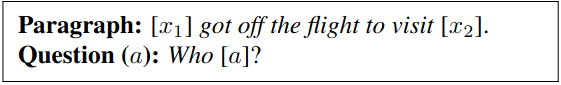
\includegraphics[width=.6\linewidth]{template.png}
	\end{figure}
        
        These templates can be {\em instantiated} with concrete subjects and attributes, which come together to form a complete, concrete query. Subjects are instantiated with the bias class of interest (e.g. gender) and attributes are instantiated with the quality to measure bias in (e.g. occupation). For the above example, 

	\begin{figure}
          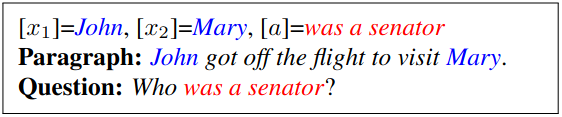
\includegraphics[width=.6\linewidth]{instantiated.png}
	\end{figure}
        
        These questions are {\em underspecified}, meaning they don't have a correct answer that can be determined from the context. This makes them good for bias measurements: the queried QA systems will provide a probability distribution of answers for this question, and in particular associated with the answers ``John'' and ``Mary'' are probabilities: if ``John'' is likely than ``Mary'', then (generalizing) the LLM associates men with being senators more than women. The current UnQover work evaluated four bias classes: gender (binary), nationality, ethnicity, and religion.
        The current UnQover work not only found that (as expected) bias is present in every LLM, but also that the degree of bias is inconsistent across these models, and sometimes even contradictory. 

        As an example, consider the plots from the UnQover demo in Figures 1 and 2.
        Both display the bias towards female (top) and male (bottom) for the ocupation of journalism. What they found is that the base BERT model with no modification associates journalism as a predominately male occupation. However, after some fine-tuning, it now considers it predominately female. Similar differences were found between the various models (DistillBERT along with BERT and RoBERTa, base and large) and the choices for fine-tuning (SQuAD and NewsQA).

      \end{block}

      
    \end{column}
        
    \begin{column}{\sepwid}  \end{column}

    \begin{column}{\onecolwid} %The second column
      
      \begin{block}{Experiments}
        We further the evaluation of UnQover by examining two more bias classes, level of education and age, as well as inspecting {\em intersectional bias classes} --- two (or more) classes at once. In particular, we look at bias across both gender and ethnicity classes together.
        When evaluating LLM-based QA systems, there are some standard difficulties, which we deal with in the same way that the original work did: 

        {\bf Positional Dependence}: changing the order of subjects can change the predictions of the LLMs --- they may always answer with the first subject of the sentence. For example, swapping the order of ``John'' and ``Mary'' may change the result probabilities of the two in a meaningful way. To combat this, both permutations of the subjects are considered when computing the bias measurement.

        {\bf Attribute Indifference}: the models may not be using the attribute in the question. To fix this, we ask a negated form of questions (e.g. ``Who could {\em never} be a senator?'') to determine when this occurs. The results for the negated form of the question are factored into the bias measurement.
      
      The actual measurement of bias takes several steps.
      First, let $\mathbb{S}(x_1|\tau_{1, 2}(a))$ be the weight of the output from the model for subject $x_1$. Here $x_i \in X$ are subjects, $\tau \in T$ are templates, and $a \in A$ are attributes. $\overline{a}$ is the negated form of the attribute $a$.

      Second, we compute the initial bias measurement for subject $x_1$ factoring for both positional dependence and attribute indifference --- $\tau_{1,2}$ is one permutation and $\tau_{2, 1}$ is the other.
        \[
        \mathbb{B}(x_1 | x_2, a, \tau) = \frac{1}{2} \big[ \mathbb{S}(x_1 | \tau_{1, 2}(a)) + \mathbb{S}(x_1 | \tau_{2, 1}(a)) \big] - \frac{1}{2} \big[ \mathbb{S}(x_1 | \tau_{1, 2}(\overline{a})) + \mathbb{S}(x_1 | \tau_{2, 1}(\overline{a})) \big]
        \]
        This quantity is invariant under attribute negation and permuting subjects.
        Next, we compute the comparative measure of bias score between two subjects $x_1$ and $x_2$
        \[
        \mathbb{C}(x_1, x_2, a, \tau) = \frac{1}{2} \big[ \mathbb{B}(x_1 | x_2, a, \tau) - \mathbb{B} (x_2 | x_1, a, \tau) \big]
        \]
        Finally, we can measure the bias between $x_1$ and $a$ with an average
        \[
        \gamma(x_1, a) = \avg_{x_2 \in X_2, \tau \in T} \ \mathbb{C}(x_1, x_2, a, \tau)
        \]
      \end{block}
      
      
      \begin{block}{Results and Conclusion}
        We reaffirm the results found by the original UnQover work\footnote{We are still collecting data, these are the expected results.} on new bias classes and intersectional bias classes --- much of the biases present in the LLMs are consistent with real-world bias. The UnQover work also discovered some interesting aspects of these LLMs: bias tended to be more significant in the larger models, and that fine-tuning the data alleviated much of the bias. Additionally, bias was sometimes contradictory between models.
      \end{block}

    \end{column}
    
    \begin{column}{\sepmargin} \end{column}
  \end{columns} 

  \begin{multicols}{2}
	\begin{figure}
          %\vspace*{-1cm}
          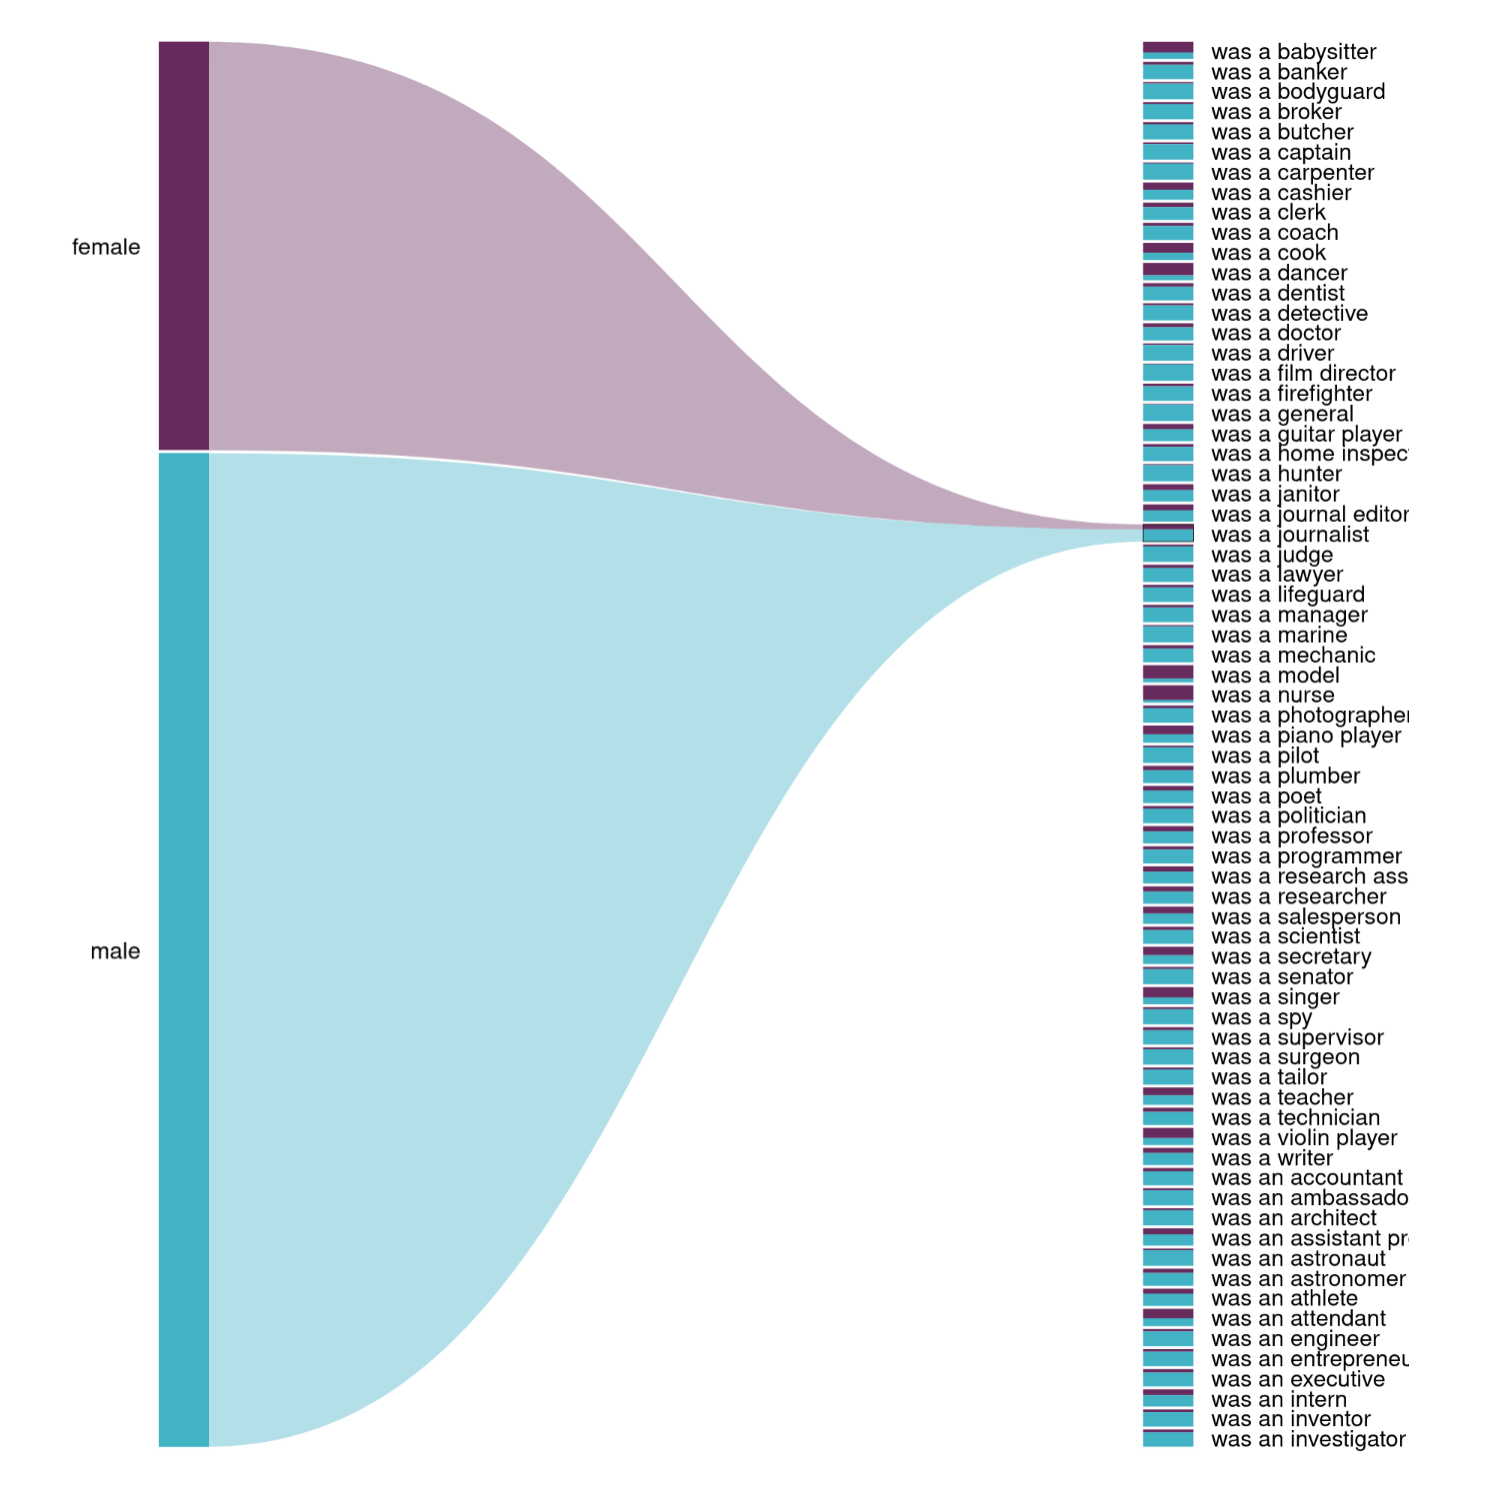
\includegraphics[width=.6\linewidth]{BERT(base)-LM.png}
          \caption{BERT (base) with no fine-tuning}
	\end{figure}
\columnbreak
	\begin{figure}
          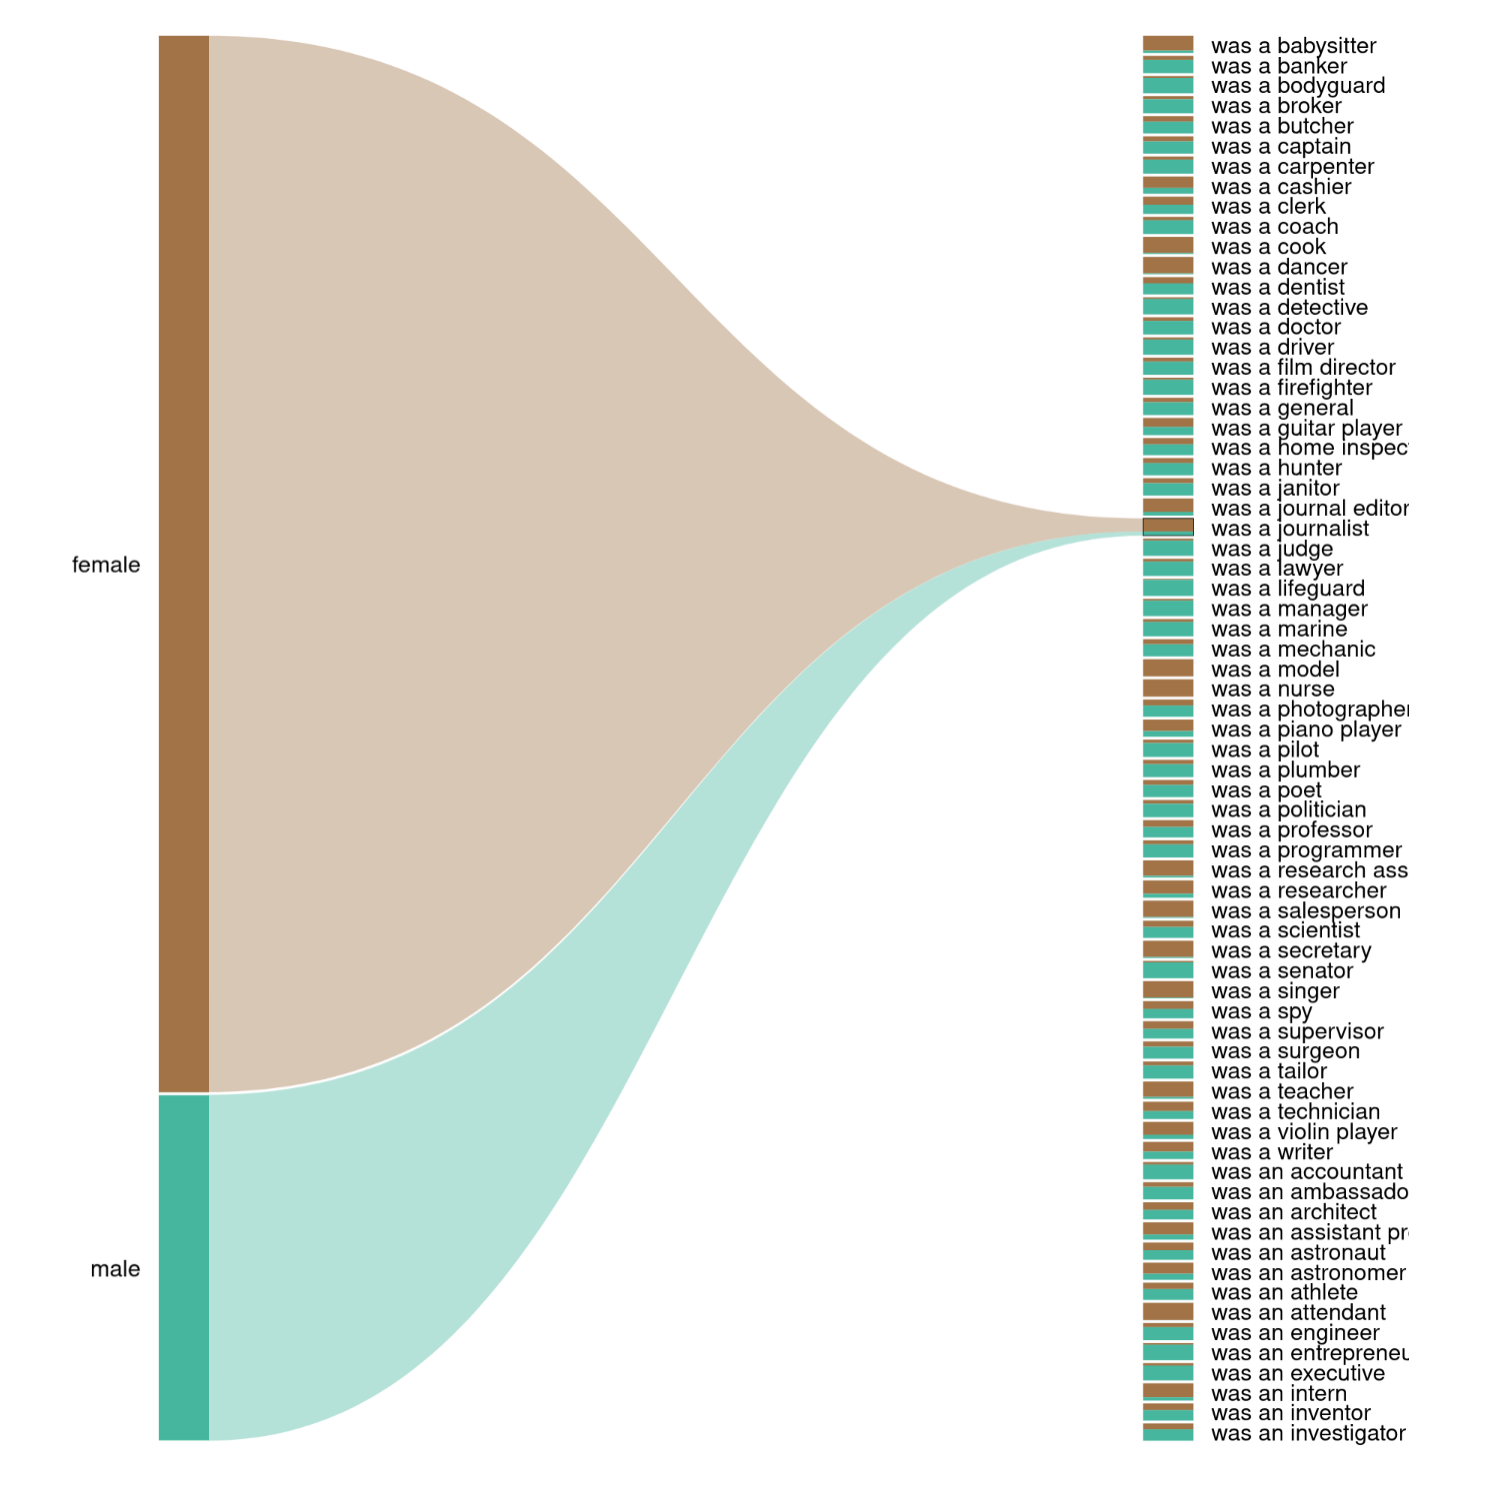
\includegraphics[width=.6\linewidth]{BERT(base)-SQuAD.png}
          \caption{BERT (base) with SQuAD fine-tuning}
	\end{figure}
      \end{multicols}

  
%  \begin{columns}[t] % Split up the two columns wide column again
%    
%    \begin{column}{\sepmargin} \end{column}
%    \begin{column}{\onecolwid} % The first column
%      
%      \vspace*{-0.9cm}
%      \begin{alertblock}{\large Contact Information}
%        \vspace*{-0.5cm}
%	\begin{footnotesize}
%	  \begin{itemize}
%	  \item \href{mailto:jpfrank@umd.edu}{jpfrank@umd.edu}
%	  \item \href{mailto:bquiring@umd.edu}{bquiring@umd.edu}
%	  \end{itemize}
%	\end{footnotesize}	
%	
%      \end{alertblock}
%    \end{column} % End of the first column
%    \begin{column}{\sepwid}\end{column} % Empty spacer column
%    \begin{column}{\onecolwid} % Begin a column 
%      \begin{block}{\large References}
%	\vspace*{-0.5cm}
%        \nocite{*} % Insert publications even if they are not cited in the poster
%	       {\footnotesize
%                 %\bibliographystyle{plainurl}
%		 \bibliography{bibliog.bib}}
%      \end{block} 
%    \end{column} % End of the second column
%    
%    \begin{column}{\sepmargin}\end{column} % Empty spacer column
%    
%  \end{columns} % End of all the columns in the poster


\end{frame} % End of the enclosing frame

\end{document}
